
\documentclass[12pt]{article}
\usepackage{amsmath}
\DeclareMathOperator*{\argmin}{arg\,min} % thin space, limits underneath in displays
\DeclareMathOperator*{\argmax}{arg\,max} % thin space, limits underneath in displays
\newtheorem{thm}{Theorem}
\usepackage{amssymb}
\usepackage{amsfonts}
\usepackage{mathrsfs}
\usepackage{bm}
\usepackage{indentfirst}
\setlength{\parindent}{0em}
\usepackage[margin=1in]{geometry}
\usepackage{graphicx}
\usepackage{setspace}
\doublespacing
\usepackage[flushleft]{threeparttable}
\usepackage{booktabs,caption}
\usepackage{float}
\usepackage{graphicx}

\usepackage{import}
\usepackage{xifthen}
\usepackage{pdfpages}
\usepackage{transparent}

\newcommand{\incfig}[1]{%
\def\svgwidth{\columnwidth}
\import{./figures/}{#1.pdf_tex}
}




\title{Notes for present value tests of an intertemporal model of the Current Account}
\author{Yan}
\date{}


\begin{document}
\maketitle
\newpage



\section{Brief Intro}

1. It shows in a simple intertemporal open economy, the current account is equal to the
expected decline of the the present discounted value of the change in net output of 
a country

\begin{align*}
CA_{t} &=  - \left( \frac{r}{1 + r}\right) 
\sum\limits_{i = 0} ^\infty \left( \frac{1}{1 + r} \right) ^{i}
{\rm I\!{E}}_{t}(NO_{t + 1} - NO_{t})\\
 &=  - \sum\limits_{i = 1} ^\infty \left( \frac{1}{1 + r} \right) 	^{i}
 {\rm I\!{E}}_{t}(\Delta NO_{t + i})
\end{align*}


2. It uses time series technique analyzing the current account for four countries. 
In two of these countries, the model works.


{\textbf {Difficulties:}} Tests are sensitive to the methods used to handle the
nonstationarities of the time series data.


With rational expectation, consumer will increase savings when expected future labor
income is expected to decrease (Campbell, 1987). In this paper, they test the similar
implication.






\section{Definition for variables}

1. Net output (NO) is defined as GDP less the sum of investment plus government spending.
\begin{equation*}
NO = Y - (I + G)
\end{equation*}

2. Discounted factor $ \beta $
\begin{equation*}
\beta = \frac{1}{1 + r}
\end{equation*}

3. Stock of external assets at the begining of period $ t + i $



\section{Theoretical Model}
\subsection{Assumptions}
1. Small open economy with a given world interest rate.

2. Consumption depends solely on a country's wealth (consumer forcasts NO).

3. The wealth is measured by the sum of NO and the stock of external assets (B).

4. The first order difference of NO is stationary, which is satisfied in the data.

5. Transversality condition:
\begin{equation}
\lim_{i \to \infty} \left( \frac{1}{1 + r} \right) ^{i}	b_{t + i} = 0, 
\end{equation}
where $ \beta = \frac{1}{1 + r} $, and $ b_{t + i} $ is the stock of external assets
at the begining of period $ t + i $.


\subsection{Model}
\subsubsection{Accumulation of external assets}
\begin{equation}
b_{t + i} = (1 + r)b_{t} + \left[ y_{t} - c_{t} - i_{t} - g_{t} \right],
\end{equation}
terms in the squared bracket is the {\textbf {trade balance (TB)}}.

Rewrite and iterate equation (2)

\begin{align*}
b_{t} &= \frac{1}{1 + r}b_{t + 1} - \frac{1}{1 + r}(y_{t} - c_{t} - i_{t} - g_{t})\\
 &= \beta b_{t + 1} -  \beta x_{t}, \text{ where $ x_{t} = y_{t} - c_{t} - i_{t} - 
 g_{t}$ is the net export }\\
 &= \beta(\beta b_{t + 2} - \beta x_{t + 1}) - \beta x_{t}\\
 &= \beta^{2} b_{t + 2} - \beta^{2} x_{t + 1}  - \beta x_{t}\\
 &...\\
\end{align*}
\begin{equation}
b_{t} =  - \sum\limits_{i = 1} ^\infty \beta^{i} x_{t + i - 1}	.
\end{equation}

It says the external asset in period $ t $ is the PDV of the stream of future trade
deficits.



\subsubsection{Agent's Intertemporal Budget constraint}
\begin{equation}
c_{t + i - 1} = y_{t + i - 1} - i_{t + i - 1} - g_{t + i - 1} - x_{t + i - 1}
\end{equation}
\begin{equation}
\sum\limits_{i = 1} ^\infty \beta^{i} c_{t + i - 1} = \sum\limits_{i = 1} ^\infty 
\beta^{i} [y_{t + i - 1} - i_{t + i - 1} - g_{t + i - 1}] - 
\sum\limits_{i = 1} ^\infty \beta^{i}x_{t + i - 1}	
\end{equation}
Plug in equation (3)
\begin{equation}
\sum\limits_{i = 1} ^\infty \beta^{i} c_{t + i - 1} =\left( 
\sum\limits_{i = 1} ^\infty 
\beta^{i} (NO)_{t + i - 1}\right) 
 + b_{t}
\end{equation}


\subsubsection{Agent's Utility function}
\begin{align*}
&U = {\rm I\!{E}}_{0}\left( \sum\limits_{i = 0} ^\infty \beta^{i} u(c_{i})	 \right)\\
& s.t. \quad
\sum\limits_{i = 1} ^\infty \beta^{i} c_{t + i - 1} =\left( 
\sum\limits_{i = 1} ^\infty 
\beta^{i} (NO)_{t + i - 1}\right) 
 + b_{t}
\end{align*}


With quadratic utility funtion, we can find the closed-form solution for consumption
\begin{equation}
c_{t} = \frac{r}{1 + r}\left\{ 
(1 + r)b_{t} + \sum\limits_{i = 0} ^\infty \left( \frac{1}{1 + r} \right)^{i}
{\rm I\!{E}}_{t}(NO_{t + i})
\right\} 
\end{equation}
They analyzed the CA with the standard rational expectations consumption function above.
\noindent\fbox{%
\parbox{\textwidth}{%
If there is a productivity shock, borrow money, $ c $ constant, $ i $ goes up,
CA deficit.

If tax rate goes up, borrow money, $ c $ constant.
}%
}\\



\subsubsection{Current Account}

\begin{equation}
CA_{t} = S_{t} - I_{t} = y_{t} + r b_{t}  - i_{t} - g_{t} - c_{t} = NO_{t} + r b_{t} - 
c_{t}
\end{equation}
Plug in equation (7)
\begin{align*}
CA_{t} &= NO_{t} + r b_{t} - \left\{ 
\frac{r}{1 + r}\left\{ 
(1 + r)b_{t} + \sum\limits_{i = 0} ^\infty \left( \frac{1}{1 + r} \right)^{i}
{\rm I\!{E}}_{t}(NO_{t + i})
\right\} 
\right\} \\
 &=  - \left( \frac{r}{1 + r} \right) \sum\limits_{i = 0} ^\infty 
 \left( \frac{1}{1 + r} \right) ^{i}{\rm I\!{E}}_{t}(NO_{t + i} - NO_{t})\\
 &=  - \sum\limits_{i = 1} ^\infty \left( \frac{1}{1 + r} \right)^{i}{\rm I\!{E}}_{t}
 (\Delta NO_{t + i}) 
\end{align*}




\section{VAR model}




The second-order VAR:
\begin{equation}
\begin{bmatrix}
\Delta NO_{t}\\
\Delta NO_{t - 1}\\
CA_{t}\\
CA_{t - 1}
\end{bmatrix}
=
\begin{bmatrix}
a_1 & a_2 & b_1 & b_2\\
1 & 0 & 0 & 0\\
c_1 & c_2 & d_1 & d_2\\
0 & 0 & 0 & 1
\end{bmatrix}
\begin{bmatrix}
\Delta NO_{t - 1}\\
\Delta NO_{t - 2}\\
CA_{t - 1}\\
CA_{t - 2}
\end{bmatrix}
 + 
\begin{bmatrix}
u_{t}\\
0\\
v_{t}\\
0
\end{bmatrix}
\end{equation}


\subsection{Restriction on VAR for $ CA_{t} $}
\subsubsection{$ \bm{K} $}
Recall
\begin{align*}
CA_{t} &=  - \sum\limits_{i = 1} ^\infty \left( \frac{1}{1 + r} \right) ^{i}
{\rm I\!{E}}_{t}(\Delta NO_{t + i})\\
\bm{CA}_{t}' &=  - \sum\limits_{i} \left( \frac{1}{1 + r} \right)^{i} \bm{h}'\bm{A}^{i}
\bm{Z}_{t}\\
 &= - \bm{h}' \sum\limits_{i} \left( \frac{\bm{A}}{1 + r} \right)^{i} \bm{Z}_{t}\\
 &= \bm{K} \bm{Z}_{t},
\end{align*}
where
\begin{equation*}
\bm{K} =  - \bm{h}' \frac{\left( \frac{A}{1 + r} \right) }{
		\left[ 1 - \left( \frac{A}{1 + r} \right)  \right] 
}.
\end{equation*}

We know $ \bm{h}' $ is a $ 1  \times 4 $ row vector, the ratio of $ \bm{A} $ is still
a $ 4  \times 4 $ matrix. Therefore, $ \bm{K} $ is a $ 1  \times 4 $ row matrix, 
$ \bm{Z_{t}} $ is a $ 4  \times  1 $ matrix,
\begin{align*}
		\bm{K} &= \begin{bmatrix}
				\gamma_1 &\gamma_2 &\gamma_3 &\gamma_4
		\end{bmatrix}\\
		\bm{Z_{t}} &= \begin{bmatrix}
				\Delta NO_{t}\\
				\Delta NO_{t - 1}\\
				CA_{t}\\
				CA_{t - 1}
		\end{bmatrix}
\end{align*}

Hence, we would like to see $ \gamma_1, \gamma_2, \text{ and } \gamma_4 $ are zeros.

Regression model could be
\begin{equation*}
CA_{t} = \gamma_1 \Delta NO_{t} + \gamma_2 \Delta NO_{t - 1} + \gamma_3 CA_{t} + 
\gamma_4 CA_{t - 1} + \eta_{t}
\end{equation*}


\subsubsection{$ \bm{R} $}
Define $ \bm{R_{t}} $ as the following
\begin{equation*}
\bm{R}_{t} = \bm{CA}_{t} - \Delta \bm{NO}_{t} - (1 + r) \bm{CA}_{t - 1}
\end{equation*}
Replace $ \bm{CA}_{t}, \bm{ \Delta NO_{t}} $ with equation in (9)
\begin{align*}
\bm{R}_{t} &= c_1 \Delta \bm{NO}_{t - 1} + c_2 \Delta \bm{NO}_{t - 2} + d_1 
\bm{CA}_{t - 1}  + d_2 \bm{CA}_{t - 2} - (a_1 \Delta \bm{NO}_{t - 1} + a_2 \Delta 
\bm{NO}_{t - 2} \\
&+ b_1 \bm{CA}_{t - 1} + b_2 \bm{CA}_{t - 2}) - (1 + r) \bm{CA}_{t - 1}\\
\bm{R}_{t}&= \varphi_1 \Delta \bm{NO}_{t - 1} + \varphi_2 \Delta \bm{NO}_{t - 2} +
\varphi_3 \bm{CA}_{t - 1} + \varphi_4 \bm{CA}_{t - 2},
\end{align*}
where 
\begin{align*}
\varphi_1  &= c_1 - a_1\\
\varphi_2 &= c_2 - a_2\\
\varphi_3 &= d_1 - b_1 - (1 + r)\\
\varphi_4 &= d_2 - b_2
\end{align*}


With information set in period $ t - 1 $, i.e., $ I_{t - 1} $, the regression model
can be 
\begin{equation*}
\bm{R}_{t}= \varphi_1 \Delta \bm{NO}_{t - 1} + \varphi_2 \Delta \bm{NO}_{t - 2} +
\varphi_3 \bm{CA}_{t - 1} + \varphi_4 \bm{CA}_{t - 2} + \varepsilon_{t}
\end{equation*}

With information set in period $ t - 2 $, i.e., $ I_{t - 2} $, the regression model
can be 
\begin{equation*}
		\bm{R}_{t} = \varphi_2 \Delta \bm{NO}_{t - 2} + \varphi_4 \bm{CA}_{t - 2} + 
		 \widetilde{\varepsilon}_{t}
\end{equation*}

But I think somewhere I did it wrong, because there is not interest rate in the model
with information set of period $ t - 2 $. The interest rate $ r $ only appears in 
$ \varphi_3 $.


The theory says $ {\rm I\!{E}}_{t - 1}(R_{t}) = 0 $, and $ {\rm I\!{E}}_{t - 2}(R_{t})
= 0$, which means we want $ \varphi_{i} = 0, \forall i = 1,2,3,4$.



\section{Data, estimation, and results}

\subsection{Data}
Four countries: Belgium, Canada, Denmark, and the United Kingdom 1955-85 data.

Net Output:
\begin{equation*}
NO = GDP - I - G,
\end{equation*}
then deflating by GDP deflator and population.

Current Account:
\begin{equation*}
CA = GNP - C - I - G,
\end{equation*}
then convert to real per capita.


\subsection{Estimation}
Check stationarity of $ \bm{NO} $ using Dickey-Fuller test.

Model:
\begin{equation*}
\Delta \bm{NO}_{t} = a + b_1 \Delta \bm{NO}_{t - 1} + b_2 \Delta \bm{NO}_{t - 2} + c
\bm{NO}_{t - 1} + d \cdot time  + \eta_{t}
\end{equation*}
It is a first difference equation with constant and deterministic trend. Construct 
$ t $-statistics and compare it with the critical value $ \tau_{\tau} $. Four columns
are for 0.01, 0.025, 0.05 0.01. We have 30 years data, therefore, $ \tau_{\tau} $ for 
5 percent level is about -3.6.

\begin{figure}[H]
\center{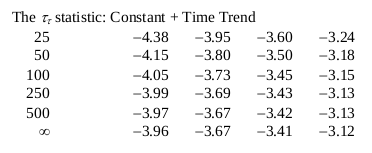
\includegraphics[scale = ]  {figures/D-F_critical_value.png}}
\end{figure}

If $ t $-statistics is on the right side of the critical value, we fail to reject the
null. Estimator $ c $ is zero with high probability.
We the net output model, we want to fail to reject the null ($ c $ = 0). For current
account we want to reject the null.

The $ t $-statistics for $ c $ among BCDU are -2.71, -2.78, 0.98, and -4.85. Except for
the UK, we fail to reject the null.

The $ t $-statistics for CA among BCDU are -2.5, -3.2, -2.1, -2.9.
The data do not show strong stationary evidence, but the authors still assume the
series are stationary.






\newpage
\subsection{Results}


\begin{figure}[H]
\center{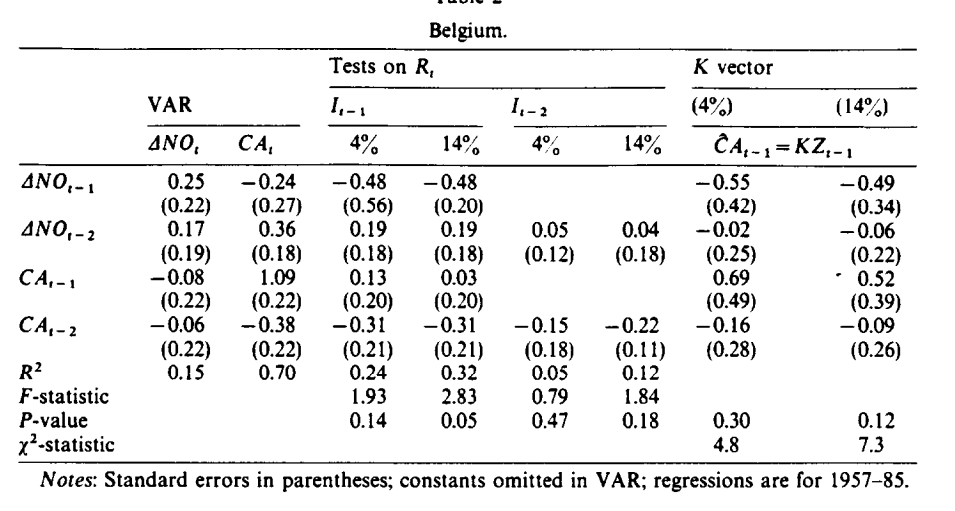
\includegraphics[scale =.5 ]  {figures/1_Belgium.png}}
\center{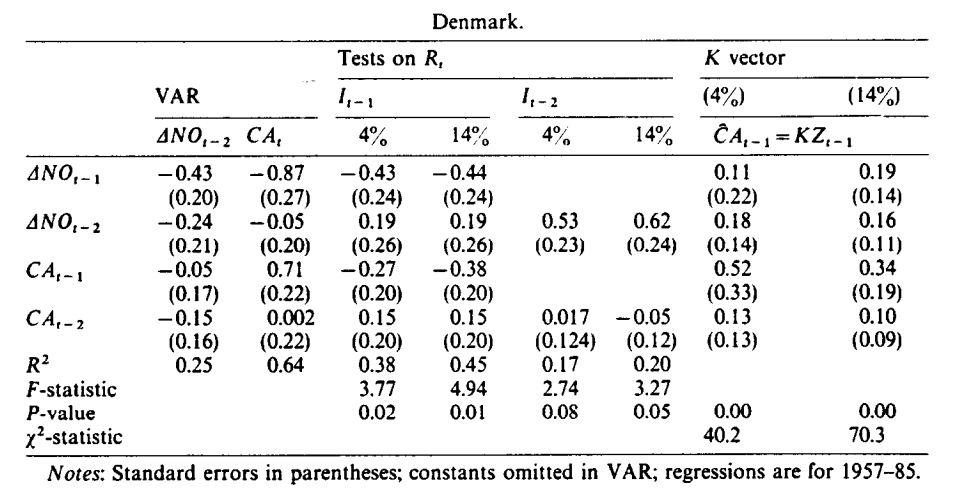
\includegraphics[scale =.5 ]  {figures/3_Denmark.png}}
\center{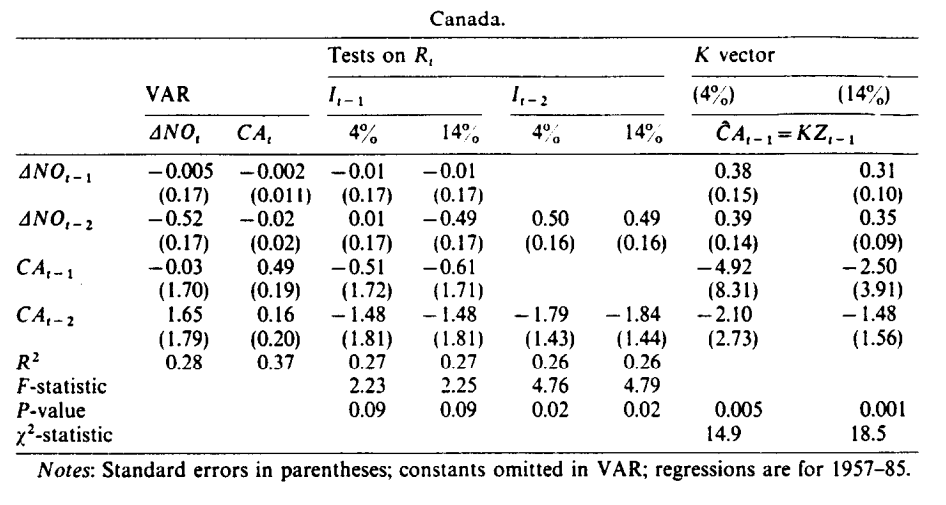
\includegraphics[scale =.5 ]  {figures/2_Canada.png}}
\end{figure}


\begin{figure}[H]
\center{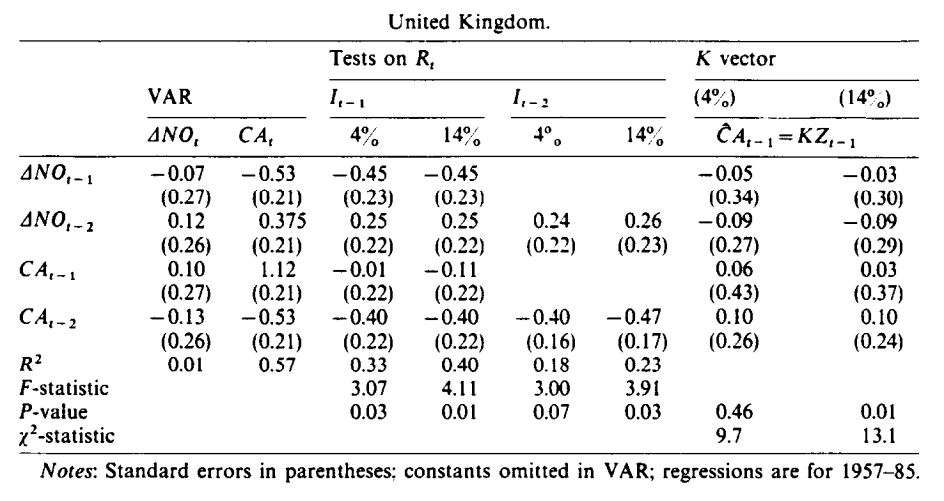
\includegraphics[scale =.5 ]  {figures/4_United_Kingdom.png}}
\end{figure}





\subsubsection{Belgium}
Belgium passes the tests on restrictions for both information sets ($ t - 1, t - 2 $) 
with $ 4\% $ interest rate. They fail to reject the null, therefore estimators are 
likely to be zeros which satisfy the model. It also passes $ I_{t - 2} $ with 
$ 14\% $ interest rate.

But the result reject the null for $ I_{t - 1} $ with $ 14\% $ interest rate.


The model for Belgium performs better at lower interest rate, consumers do not discount
the future very heavily, place too little weight on current income.


\subsubsection{Denmark}
Test on Information set:

$ I_{t - 1} $ rejects the null with $ 5\% $ level, and $ I_{t - 2} $ rejects the
null with $ 10\% $ level.
It performs slightly better with lower interest rate.

$ \bm{K} $ vector:
It performs well, and is close to $ [0 \quad 0 \quad 1 \quad 0] $.
The estimated CA trend with $ \bm{K} $ vector match the real data well.


\subsubsection{UK and Canada}
The model fits these two countries poorly.

{\textbf {Canada:}}

The data reject the null with $ 5\% $ level for $ I_{t - 2} $, and with $ 10\% $ level
for $ I_{t - 1} $. The estimators are far away from zero.

$ \bm{K} $ vector: far away from 0 and 1.


{\textbf {UK:}}

The data reject the null with $ 5\% $ level for $ I_{t - 1} $ and $ I_{t - 2} $ with
$ 14\% $ interest rate. And they reject the null with $ 10\% $ level for $ I_{t - 2} $
with $ 4\% $ interest rate.


$ \bm{K} $ vector: estimators are all close to zero.















\end{document}

